% polynome
%-------------------
% Teiler für das Skalieren der Grafik /40
\newcommand{\teiler}{40}


%//////////////////////////////////////

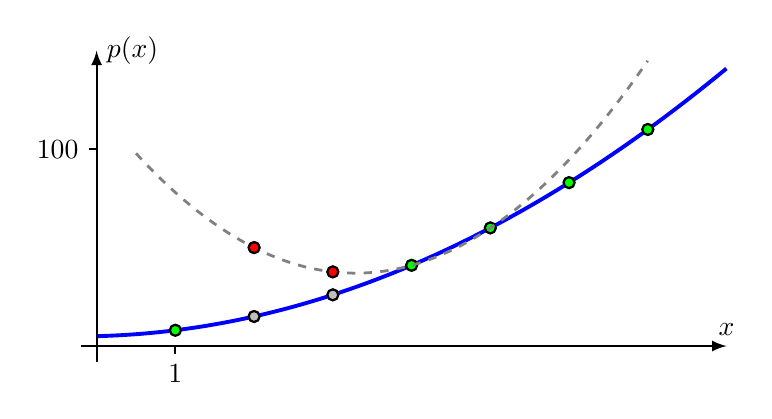
\begin{tikzpicture}[>=latex,thick]
	\draw[color=blue, line width=1.4pt] 
	plot[domain=0:8, samples=100]
	({\x},{(2*\x^2+1*\x+5)/\teiler});

	\draw[->] (-0.2,0) -- (8,0) coordinate[label={$x$}];
	\draw[->] (0,-0.2) -- (0,150/\teiler) coordinate[label={right:$p(x)$}];
	
	\def\punkt#1{
		\fill[color=green] #1 circle[radius=0.08];
		\draw #1 circle[radius=0.07];
	}

	\def\hellpunkt#1{
		\fill[color=lightgray] #1 circle[radius=0.08];
		\draw #1 circle[radius=0.07];
	}
	
	\punkt{(1,8/\teiler)}
	\hellpunkt{(2,15/\teiler)}
	\hellpunkt{(3,26/\teiler)}
	\punkt{(4,41/\teiler)}
	\punkt{(5,60/\teiler)}
	\punkt{(6,83/\teiler)}
	\punkt{(7,110/\teiler)}
	
	\draw[color=gray,line width=1pt,dashed] 
	plot[domain=0.5:7, samples=100]
	({\x},{(7.832*\x^2-51.5*\x+121.668)/\teiler});
	
	\def\erpunkt#1{
		\fill[color=red] #1 circle[radius=0.08];
		\draw #1 circle[radius=0.07];
	}
	\erpunkt{(2,50/\teiler)}
	\erpunkt{(3,37.66/\teiler)}

	\draw(0,100/\teiler) -- (-0.1,100/\teiler) coordinate[label={left:$100$}];
	\draw(1,0) -- (1,-0.1) coordinate[label={below:$1$}];		
\end{tikzpicture}
%\end{document}
